

%%%-------------------------------------------------------------------
\section{Introdução}
\label{intro}

\begin{frame}
\frametitle{Dados de contagens}
Alguns exemplos de problemas envolvendo contagens:

\vspace{0,2cm}
\begin{itemize}
\item Número de acidentes em uma rodovia por semana;
\item Número de automóveis vendidos por dia;
\item Número de gols marcados por times de futebol por partida;
\item Número de falhas por metro de fio de cobre produzido;
\item Número de colônias de bactérias por $0,01mm^{2}$ de uma dada 
cultura $\ldots$

\end{itemize}
\end{frame}
%%%-------------------------------------------------------------------

\begin{frame}
\frametitle{Modelos probabilísticos para dados de contagens}

\begin{itemize}
    \item Modelos probabilísticos para variáveis aleatórias discretas, 
    com suporte no conjunto de números inteiros não-negativos, 
    são potenciais candidatos para a análise de dados de contagens.
\vspace{0.5cm}
    \item Algumas alternativas: Distribuição Binomial, Poisson e 
    generalizações; distribuições geradas por misturas, como a 
    beta-binomial, binomial negativa; distribuições fundamentadas na 
    modelagem do tempo entre eventos, na razão de probabilidades 
    sucessivas $\ldots$

\end{itemize}
\end{frame}

%%%-------------------------------------------------------------------
\begin{frame}\frametitle{Regressão para dados de contagens}

\begin{itemize}

\item Modelos de regressão são utilizados para modelar a distribuição 
de uma variável aleatória $Y$ condicional aos valores de um conjunto 
de variáveis explicativas $x_{1},x_{2},...,x_{p}$.

\vspace{0,5cm}

\item Métodos para inferência e modelos de regressão para dados de 
contagem estão aquém, em quantidade e diversidade, em relação ao 
verificado para dados contínuos.

\vspace{0,5cm}

\item A aplicação de modelos de regressão com erros normais na análise 
de contagens, embora frequente, em geral é desaconselhável.

\end{itemize}
\end{frame}

%%%-------------------------------------------------------------------
\begin{frame}{Regressão com erros normais na análise de dados de contagens}
    \vspace{0,5cm}

    \begin{itemize}
        \item O modelo linear com erros normais não considera a 
        natureza discreta dos dados;
        \vspace{0,5cm}
        \item Associa probabilidade nula a qualquer possível contagem;
        \vspace{0,5cm}
        \item Admite probabilidades não nulas a valores negativos 
        da variável;
    \end{itemize}

\end{frame}

%%%-----------------------------------------------------------------------------------------
\begin{frame}{Regressão com erros normais na análise de dados de contagens}
     \vspace{0,2cm}
 
    \begin{itemize}
        \item O uso de transformações dificulta a interpretação dos 
        resultados;
        \vspace{0,5cm}
        \item O uso da transformação logarítmica apresenta problemas 
        para contagens iguais a zero;
        \vspace{0,5cm}
        \item Não se contempla a relação não constante entre variância
        e média, característica de  dados de contagens.
    \end{itemize}

\end{frame}

%%%-------------------------------------------------------------------
\begin{frame}{A distribuição de Poisson}

    \begin{itemize}
        \item A distribuição de Poisson é a principal referência para 
        a análise de dados de contagens.
    \vspace{0,3cm}
        \item Função de probabilidades:
$$
P\left (Y=k \right )=\frac{e^{-\mu}\mu^{k}}{k!},\quad k = 0, 1, 2, \ldots; \mu>0.
$$
   \vspace{0,2cm}
       \item Se os eventos sob contagem  ocorrem independentemente e 
       sujeitos a uma taxa constante $\mu >0$, sob o modelo Poisson,  
       para um intervalo de exposição de tamanho $t$ tem-se:

$$
    P\left ( Y_t = k \right)=\frac{e^{-\mu t}(\mu t)^{k}}{k!}, \quad k = 0,1,2,\ldots
$$
        \end{itemize}

\end{frame}

%%%-------------------------------------------------------------------
\begin{frame}{Propriedades da distribuição de Poisson}

Dentre as principais propriedades da distribuição de Poisson, tem-se:
\vspace{0,3cm}
\begin{itemize}

    \item Média: $E(Y)= \mu$;
    \vspace{0,5cm}
    \item Variância: $Var(Y)=\mu$ (equidispersão);
    \vspace{0,5cm}
    \item Razão de probabilidades sucessivas: 
    $\frac{P\left ( X=k \right )}{P\left ( X=k-1 \right )}=\frac{\lambda}{k},$ 
    gerando a relação de recorrência:
    $$
        P(Y=k)k=P(Y=k-1)\lambda;
    $$
    \item Se $Y_{1},Y_{2},...,Y_{n}$ são v.a.s independentes com 
    $Y_{i}\sim Poisson(\lambda_{i})$, e $\sum\mu_{i}<\infty$, então 
    $\sum Y_{i}\sim Poisson(\sum\mu_{i})$.
    \end{itemize}
\end{frame}

%%%-------------------------------------------------------------------

\begin{frame}{Motivações para a distribuição de Poisson}

\begin{itemize}
\item Se o tempo decorrido entre sucessivos eventos é uma variável 
aleatória com distribuição exponencial de média $\lambda=1/\mu$, 
então o número de eventos ocorridos em um intervalo $t$ de tempo tem 
distribuição de Poisson com média $\mu t$.

\vspace{0,3cm}
\begin{itemize}
\item A dualidade entre as distribuições Poisson e exponencial implica 
que a taxa de ocorrência do evento, definida por:
\end{itemize}
$$
\mu(t) =\lim_{\Delta t\rightarrow 0}\frac{P\left \{ \text{evento ocorrer em} 
\left ( t,t+\Delta t \right ) \right \}}{\Delta t},
$$
\vspace{0,3cm}
dado que o evento não ocorreu até o tempo $t$, \textbf{é constante} 
para todo $t>0$.
\end{itemize}
\end{frame}
%%%-------------------------------------------------------------------
\begin{frame}{Diferentes comportamentos para $\mu(t)$}
  \vspace{-1.5cm}
  \begin{figure}[h]
  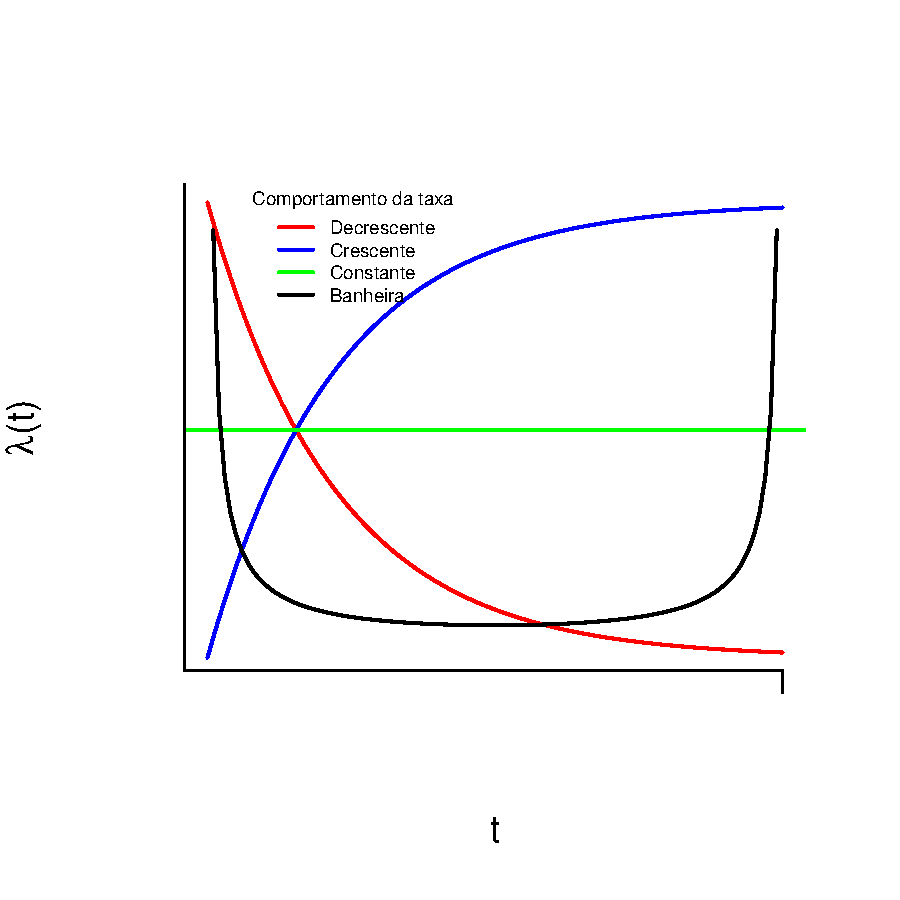
\includegraphics[height=8cm,width=10cm]{images/Graf_Risco.pdf}
  \vspace{-0.8cm}
  \caption{Diferentes comportamentos para $\mu(t)$}
  %% \label{Fig1}
  \centering
\end{figure}
\end{frame}
%%%-------------------------------------------------------------------
\begin{frame}{O processo de Poisson}
O Processo de Poisson configura um processo de contagem em que 
$Y(t),t\geqslant 0$, representa o número de eventos que ocorrem até $t$, 
satisfazendo:
\vspace{0,5cm}
\begin{enumerate}
  \item $Y(t)$ é inteiro e não negativo;
  \item Para $s<t$, $Y(s)\leq Y(t)$;
  \item $Y(t)-Y(s)$ é o número de eventos que ocorrem no intervalo $(s,t]$;
\item O processo é estacionário:

$$
  Y(t_{2}+s)-Y(t_{1}+s) \overset{i.d. }{\sim}Y(t_{2})-Y(t_{1}), \forall s>0
$$
  
\item O processo tem incrementos independentes, ou seja, os números de 
eventos verificados em intervalos disjuntos são independentes.
\end{enumerate}

\end{frame}

%%%-------------------------------------------------------------------
\begin{frame}{Diferentes padrões em processos de contagens}

\begin{figure}[h]
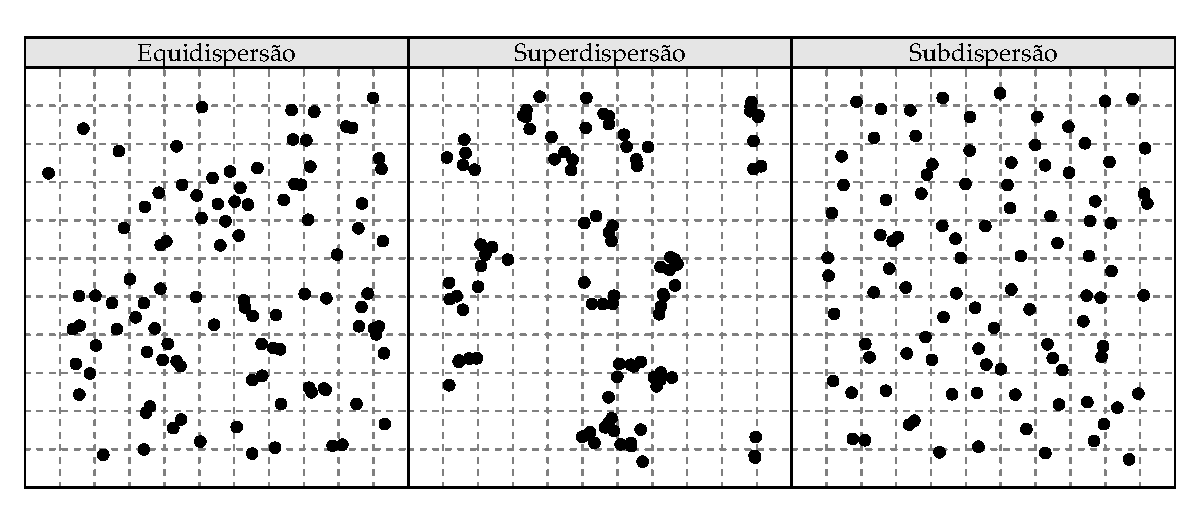
\includegraphics[scale=0.6]{images/processos14.pdf}
\caption{Ilustração de diferentes tipos de processos pontuais}
\label{Fig2}
\centering

\end{figure}
\end{frame}

%%%-------------------------------------------------------------------
\begin{frame}{O desafio de dados de contagem}
\begin{itemize}
\item Poisson implica equidispersão, ou seja,
$$ E(Y) = var(Y) = \mu. $$
\item Na prática podemos ter
\begin{itemize}
  \item Sub dispersão $E(Y) > var(Y)$;
  \item Super dispersão $E(Y) < var(Y)$.
\end{itemize}
  \item Implicações: distribuições com mais ou menos zeros e caldas
  mais leves ou pesadas comparadas com o modelo de Poisson.

\end{itemize}

\end{frame}
